\section{Custom Elements}\label{custom-elements}

Webseiten werden mit sogenannten Elementen, oder auch Tags, aufgebaut. Das Set an verfügbaren Elementen wird vom \ac{W3C} definiert und standardisiert. Somit ist die Auswahl an den verfügbaren Elementen stark begrenzt und nicht von Entwicklern erweiterbar, sodass diese ihre eigenen, von ihrer Applikation benötigten Elemente, definieren können. Betrachtet man in Abbildung \ref{fig:cusel} den Quelltext einer populären Webseite im Internet, wird schnell deutlich, worin das Problem liegt.

\begin{figure}[htbp]
 \centering
 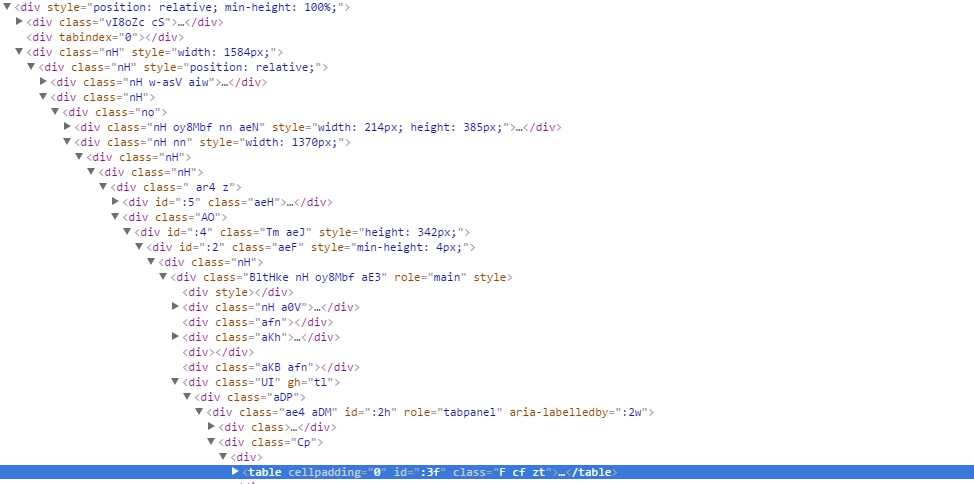
\includegraphics[width=\linewidth]{kapitel2/bilder/2-custom-elements-div-suppe}
 \caption{Webseite mit semantisch nicht aussagekräftigem Markup}
 \label{fig:cusel}
\end{figure}

Die Webseite der Google Mail Applikation ist stark geschachtelt in \texttt{\textless{}div\textgreater{}}-Elemente. Diese sind notwendig, um der Webseite die gewünschte Funktionalität und Aussehen zu verleihen. Die Probleme dieser Struktur bzw. des \ac{DOM}s sind deutlich: Es ist sehr schwer zu erkennen, welches Element nun was darstellt und welche Funktion hat. Abgesehen von der fehlenden schnell ersichtlichen Semantik - also der Zuordnung der Bedeutung zu einem Element - ist das gesamte \ac{DOM} nur schwer wartbar.

Dieser Problematik widmen sich die Custom Elements. Sie bieten eine neue \ac{API}, welche es ermöglicht, eigene, semantisch aussagekräftige \ac{HTML}-Elemente sowie deren Eigenschaften und Funktionen zu definieren. Würde das obige Beispiel nun also mit Hilfe von Custom Elements umgesetzt werden, so könnte das zugehörige \ac{DOM} wie in Listing \ref{beamwc} dargestellt aussehen \cite{citeulike:13844982}.

\lstinputlisting[language=HTML,label=beamwc,caption=Beispiel einer Applikation mit Web Components]{kapitel2/listings/2-1.html}

Die Spezifikation des \ac{W3C} ermöglicht nicht nur das Erstellen eigenständiger Elemente, sondern auch das Erstellen von Elementen, welche native Elemente erweitern. Somit können die \ac{API}s von nativen \ac{HTML}-Elementen um eigene Eigenschaften und Funktionen erweitert werden. Dies ermöglicht es, gewünschte Funktionalitäten in selbsterstellten \ac{HTML}-Elementen zu bündeln.


\subsection{Neue Elemente registrieren}\label{neue-elemente-registrieren}

Um nun ein eigenes Custom Element zu definieren, muss der Name des Custom Elements laut der \ac{W3C} Spezifikation zwingend einen Bindestrich enthalten, beispielsweise \texttt{my-element}. Somit ist gewährleistet, dass der Parser des Browsers die Custom Elements von den nativen Elementen unterscheiden kann \cite{citeulike:13845061}. Ein neues Element wird mittels JavaScript mit der Funktion \texttt{var\ MyElement\ =\ document.registerElement('my-element');} registriert. Zusätzlich zum Namen des Elements kann optional der Prototyp des Elements angegeben werden. Dieser ist jedoch standardmäßig ein \texttt{HTMLElement}, somit also erst wichtig, wenn es darum geht, vorhandene Elemente zu erweitern, auf dieses Thema wird jedoch in Abschnitt \ref{vorhandene-elemente-erweitern-type-extensions} gesondert eingegangen. Durch das Registrieren des Elements wird es in die Registry des Browsers geschrieben, welche dazu verwendet wird, die Definitionen der \ac{HTML}-Elemente aufzulösen. Nachdem das Element registriert wurde, muss es zunächst mittels \texttt{document.createElement(tagName)} erzeugt werden, der \texttt{tagName} ist hierbei der Name des zuvor registrierten Elements. Danach kann es per JavaScript mittels \texttt{document.body.appendChild(myelement);} oder per \ac{HTML}-Deklaration mittels \texttt{\textless{}my-element\textgreater{}\textless{}my-element\textgreater{}} im Dokument verwendet werden \cite[S. 127-138]{citeulike:13844975}.


\subsection{Vorteile von Custom Elements}\label{vorteile-von-custom-elements}

Ist ein Element noch nicht definiert und nicht beim Browser registriert, steht aber im Markup der Webseite, beispielsweise \texttt{\textless{}myelement\textgreater{}}, wird dies kein Fehler verursachen, da dieses Element das Interface von \texttt{HTMLUnkownElement} benutzen muss \cite{citeulike:13851253}. Ist es jedoch definiert oder beim Browser registriert worden, beispielsweise mit \texttt{\textless{}my-element\textgreater{}}, so benutzt es das Interface eines \texttt{HTMLElement}. Dies bedeutet, dass für dieses Element eigene \ac{API}s erzeugt werden können, indem eigene Eigenschaften und Methoden hinzugefügt werden \cite{citeulike:13844982}. Eigene Elemente mit einem spezifischen Eigenverhalten und Aussehen, wie beispielsweise ein neuer Video-Player, sind dadurch mit einem Tag statt mit einem Gerüst aus \texttt{\textless{}div\textgreater{}}-Tags oder Ähnlichem umsetzbar.


\subsection{Nachteil}\label{nachteile-von-custom-elements}

Ein Custom Element, welches zwar standardkonform deklariert oder erstellt, aber noch nicht beim Browser registriert wurde, ist ein ``Unresolved Element''. Steht dieses Element am Anfang des \ac{DOM}, wird jedoch erst später registriert, kann es nicht von \ac{CSS} angesprochen werden. Dadurch kann ein \ac{FOUC} entstehen, was bedeutet, dass das Element beim Laden der Seite nicht gestylt dargestellt wird, sondern das definierte Aussehen erst übernimmt, nachdem es registriert wurde. Um dies zu verhindern, sieht die \ac{HTML}-Spezifikation eine neue \ac{CSS}-Pseudoklasse \texttt{:unresolved} vor, welche deklarierte, aber nicht registrierte Elemente anspricht. Somit können diese Elemente initial beim Laden der Seite ausgeblendet und nach dem Registrieren wieder eingeblendet werden. Dadurch wird ein ungewolltes Anzeigen von ungestylten Inhalten verhindert \cite{citeulike:13844984}.


\subsection{Vorhandene Elemente erweitern (Type Extensions)}\label{vorhandene-elemente-erweitern-type-extensions}

Statt neue Elemente zu erzeugen können sowohl native \ac{HTML}-Elemente als auch bereits erstellte Custom Elements durch prototypische Vererbung um Funktionen und Eigenschaften erweitert werden, was auch als ``Type Extension'' bezeichnet wird. Zusätzlich zum Namen des erweiterten Elements wird nun der Prototyp sowie der Name des zu erweiternden Elements der \texttt{registerElement}-Funktion als Parameter übergeben. Soll also ein erweitertes \texttt{button}-Element registriert werden, muss dies wie in Listing \ref{reebe} gemacht werden:

\lstinputlisting[language=JavaScript,label=reebe,caption=Registrieren eines erweiterten Button-Elements]{kapitel2/listings/2-2.js}

Das registrierte, erweiterte Element kann nun mit dem Namen des zu erweiternden Elements als erstem Parameter und dem Namen des erweiterten Elements als zweitem Parameter erzeugt werden. Alternativ kann es auch mit Hilfe des Konstruktors erzeugt werden (siehe Listing \ref{eeebe}) \cite{citeulike:13752379}.

\lstinputlisting[language=HTML,label=eeebe,caption=Erzeugen eines erweiterten Button-Elements]{kapitel2/listings/2-3.js}

Um es nun im \ac{DOM} zu benutzen, muss der Name des erweiterten Elements via dem Attribut \texttt{is=\dq elementName\dq} des erweiternden Elements angegeben werden. So wird der erweiterte Button deklarativ mittels \texttt{\textless{}button\ is=\dq button-extended\dq\textgreater{}\textless{}/button\textgreater{}} in das Dokument eingebunden.


\subsection{Eigenschaften und Methoden definieren}\label{eigenschaften-und-methoden-definieren}

Anhand des Beispiels auf GitHub wird deutlich, wie ein Custom Element eingesetzt werden kann, jedoch sind die internen JavaScript Mechanismen nicht ersichtlich. Custom Elements entfalten ihr vollständiges Potential jedoch erst, wenn man für diese auch eigene Eigenschaften und Methoden definiert. Wie bei nativen \ac{HTML}-Elementen ist das auch bei Custom Elements auf analoge Weise möglich \cite[S. 127-138]{citeulike:13844975}. So kann einem Element eine Funktion zugewiesen werden, in dem diese dessen Prototyp mittels einem nicht reservierten Namen angegeben wird. Selbiges gilt für eine neue Eigenschaft. Die Eigenschaften können, nachdem sie im Prototyp definiert wurden, im \ac{HTML}-Markup deklarativ konfiguriert werden (siehe Listing \ref{eumduk}).

\lstinputlisting[language=HTML,label=eumduk,caption=Eigenschaften und Methoden definieren und konfigurieren]{kapitel2/listings/2-4.html}


\subsection{Custom Element Lifecycle-Callbacks}\label{custom-element-lifecycle-callbacks}

Custom Elements bieten eine standardisierte \ac{API} an speziellen Methoden, den ``Custom Element Lifecycle-Callbacks'', welche es ermöglichen Funktionen zu unterschiedlichen Zeitpunkten - vom Registrieren bis zum Löschen eines Custom Elements - auszuführen. Diese ermöglichen es, zu bestimmen, wann und wie ein bestimmter Code des Custom Elements ausgeführt werden soll.

\textbf{createdCallback}

Die \texttt{createdCallback}-Funktion Wird ausgeführt, wenn eine Instanz des Custom Elements mittels \texttt{var\ mybutton\ =\ document.createElement('custom-element')} erzeugt wurde.

\textbf{attachedCallback}

Die \texttt{attachedCallback}-Funktion wird ausgeführt, wenn ein Custom Element dem \ac{DOM} mittels \texttt{document.body.appendChild(mybutton)} angehängt wurde.

\textbf{detachedCallback}

Die \texttt{detachedCallback}-Funktion wird ausgeführt, wenn ein Custom Element aus dem \ac{DOM} mittels \texttt{document.body.removeChild(mybutton)} entfernt wurde.

\textbf{attributeChangedCallback}

Die \texttt{attributeChangedCallback}-Funktion wird ausgeführt, wenn ein Attribut eines Custom Elements mittels \texttt{MyElement.setAttribute()} geändert wurde.

So können die Lifecycle-Callbacks für ein neues erweitertes Button-Element, wie in Listing \ref{lccdebd} dargestellt, definiert werden \cite{citeulike:13844988}.

\lstinputlisting[language=HTML,label=lccdebd,caption=Lifecycle-Callbacks des erweiterten Buttons definieren]{kapitel2/listings/2-5.html}


\subsection{Styling von Custom Elements}\label{styling-von-custom-elements}

Das Styling von eigenen Custom Elements funktioniert analog dem Styling von nativen \ac{HTML}-Elementen indem der Name des Elements als \ac{CSS}-Selektor angegeben wird (siehe Listing \ref{seceudeb}). Erweiterte Elemente können mittels dem Attribut-Selektor in \ac{CSS} angesprochen werden \cite[S. 127-138]{citeulike:13844975}.

\lstinputlisting[language=HTML,label=seceudeb,caption=Styling eines Custom Element und des erweiterten Button]{kapitel2/listings/2-6.css}


\subsection{Verwendung bei GitHub}\label{verwendung-bei-github}

Eine Umsetzung der Type extensions ist auf der Webseite von GitHub zu finden. Dort werden die ``Latest commit'' Angaben eines Repositories als ein erweitertes \texttt{time}-Element dargestellt. Statt des Commit-Datums und der Zeit, wird die berechnete Zeit seit dem letzten Commit angezeigt, wie in Abbildung \ref{fig:ghece} dargestellt.

\begin{figure}[htbp]
 \centering
 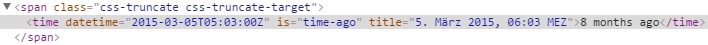
\includegraphics[width=\linewidth]{kapitel2/bilder/2-custom-elements-github-time-element}
 \caption{Github Einsatz eines Custom Element}
 \label{fig:ghece}
\end{figure}

GitHub verwendet hierzu ein selbst erzeugtes \texttt{time-ago}-Element, welches eine Type extension auf Basis des `time`-Elements umsetzt. Mittels dem \texttt{datetime}-Attribut wird die absolute Zeit des Commits an das interne JavaScript weitergegeben. Als Inhalt des \texttt{time}-Elements wird dann die mit JavaScript berechnete relative Zeit ausgegeben. Falls der Browser nun keine Custom Elements unterstützt oder JavaScript deaktiviert ist, wird dennoch das nicht erweiterte, native HTML \texttt{time}-Element mit der absoluten Zeit angezeigt.


\subsection{Browserunterstützung}\label{custom-elements-browserunterstuetzung}

Custom Elements sind noch nicht vom \ac{W3C} standardisiert, sondern befinden sich noch im Status eines ``Working Draft'' \cite{citeulike:13845061}. Sie werden deshalb bisher nur von Google Chrome ab Version 43 und Opera ab Version 33 nativ unterstützt (siehe Abbildung \ref{fig:buce}) \cite{citeulike:13844983}.

\begin{figure}[htbp]
 \centering
 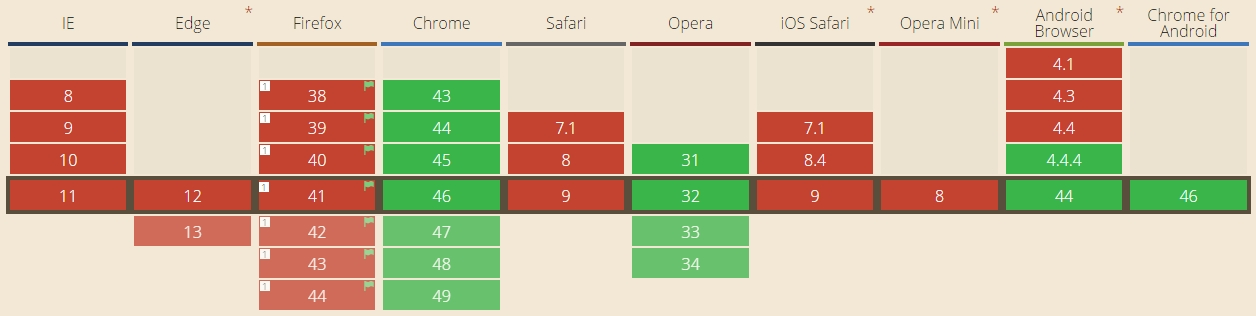
\includegraphics[width=\linewidth]{kapitel2/bilder/2-custom-elements-browserunterstuetzung}
 \caption{Browserunterstützung von Custom Elements}
 \label{fig:buce}
\end{figure}
